%\ chapters/ce1-2025-problems.tex
% GATE CE1 - Problems (BT25 format)
% Compile with XeLaTeX. Main language = English, Arabic only in heading.
% Each problem is an \item of the outer enumerate.
% Options are a nested enumerate so they are NOT numbered as problems.

\section*{\textarabic{المسائل}}    % "Problems" (only Arabic text in the document)
\setcounter{subsection}{1}         % labels become 1.1, 1.2, ...

\begin{enumerate}[label=\thesubsection.\arabic*, ref=\thesubsection.\theenumi, itemsep=0pt, leftmargin=*]

% ----------------------------------------------------------- Q3
\item At how many points will the curves $y = x^2$ and $y = -x^2 - 2x - 1$ intersect in the real $\brak{x,y}$ plane? \gate
\begin{multicols}{2}
\begin{enumerate}[label=\alph*), itemsep=0pt]
\item 0
\item 1
\item 2
\item 3
\end{enumerate}
\end{multicols}
\solution Writing both curves in the form \eqref{eq:conic},
\begin{align}
x^2 - y = 0 &\implies \vec{V}_1 = \myvec{1 & 0\\ 0 & 0},\ \vec{u}_1 = \myvec{0\\ -\frac{1}{2}},\ f_1 = 0\\
x^2 + 2x + y + 1 = 0 &\implies \vec{V}_2 = \myvec{1 & 0\\ 0 & 0},\ \vec{u}_2 = \myvec{1\\ \frac{1}{2}},\ f_2 = 1
\end{align}
Using \eqref{eq:class},
\begin{align}
\abs{\vec{V}_1} = \mydet{1 & 0\\ 0 & 0} = 0,\quad \abs{\vec{V}_2} = \mydet{1 & 0\\ 0 & 0} = 0
\end{align}
so both curves are parabolas. Any common point lies on every member of the pencil \eqref{eq:pencil}:
\begin{align}
\vec{x}^\top\myvec{1+\mu & 0\\ 0 & 0}\vec{x} + 2\myvec{\mu\\ \frac{\mu-1}{2}}^\top\vec{x} + \mu = 0
\end{align}
The pencil is degenerate when \eqref{eq:degen} holds. Expanding along the second row using \eqref{eq:detexp} and \eqref{eq:det2},
\begin{align}
\mydet{1+\mu & 0 & \mu\\ 0 & 0 & \frac{\mu-1}{2}\\ \mu & \frac{\mu-1}{2} & \mu}
&= -\frac{\mu-1}{2}\mydet{1+\mu & 0\\ \mu & \frac{\mu-1}{2}}\\
&= -\frac{\brak{\mu-1}^2\brak{\mu+1}}{4} = 0 \implies \mu = -1,\ \mu = 1
\end{align}
For $\mu = -1$, $\vec{V}_1 - \vec{V}_2 = \vec{0}$ and the second-degree terms vanish. From \eqref{eq:chord},
\begin{align}
2\brak{\vec{u}_1 - \vec{u}_2}^\top\vec{x} + \brak{f_1 - f_2} &= 0\\
2\myvec{-1 & -1}\vec{x} - 1 = 0 &\implies \myvec{1 & 1}\vec{x} = -\frac{1}{2}
\end{align}
The normal vector is $\vec{n} = \myvec{1\\ 1}$. From \eqref{eq:normal} and \eqref{eq:lineform}, a point on the line and its direction vector are
\begin{align}
\vec{h} = \myvec{0\\ -\frac{1}{2}},\quad \vec{m} = \myvec{1\\ -1},\quad \vec{x} = \vec{h} + \kappa\vec{m}
\end{align}
Substituting this line into the first parabola using \eqref{eq:quadk} and \eqref{eq:gh},
\begin{align}
\vec{m}^\top\vec{V}_1\vec{m} &= \myvec{1 & -1}\myvec{1 & 0\\ 0 & 0}\myvec{1\\ -1} = 1\\
\vec{V}_1\vec{h} + \vec{u}_1 &= \myvec{1 & 0\\ 0 & 0}\myvec{0\\ -\frac{1}{2}} + \myvec{0\\ -\frac{1}{2}} = \myvec{0\\ -\frac{1}{2}}\\
\vec{m}^\top\brak{\vec{V}_1\vec{h} + \vec{u}_1} &= \myvec{1 & -1}\myvec{0\\ -\frac{1}{2}} = \frac{1}{2}\\
g\brak{\vec{h}} &= \vec{h}^\top\vec{V}_1\vec{h} + 2\vec{u}_1^\top\vec{h} + f_1 = 0 + \frac{1}{2} + 0 = \frac{1}{2}
\end{align}
which gives
\begin{align}
\kappa^2 + \kappa + \frac{1}{2} = 0
\end{align}
The discriminant from \eqref{eq:disc} is
\begin{align}
\Delta = \sbrak{\vec{m}^\top\brak{\vec{V}_1\vec{h} + \vec{u}_1}}^2 - g\brak{\vec{h}}\brak{\vec{m}^\top\vec{V}_1\vec{m}} = \frac{1}{4} - \frac{1}{2} = -\frac{1}{4} < 0
\end{align}
From \eqref{eq:kappa},
\begin{align}
\kappa = -\frac{1}{2} \pm \frac{j}{2}
\end{align}
which is not real (here j is iota). As a check, the other degenerate member $\mu = 1$ gives
\begin{align}
\brak{x^2 - y} + \brak{x^2 + 2x + y + 1} = 2x^2 + 2x + 1 = 0 \implies x = \frac{-1 \pm j}{2}
\end{align}
which is again not real. Hence the curves do not meet in the real $\brak{x,y}$ plane and the number of intersection points is $0$.

\begin{figure}[H]
\centering
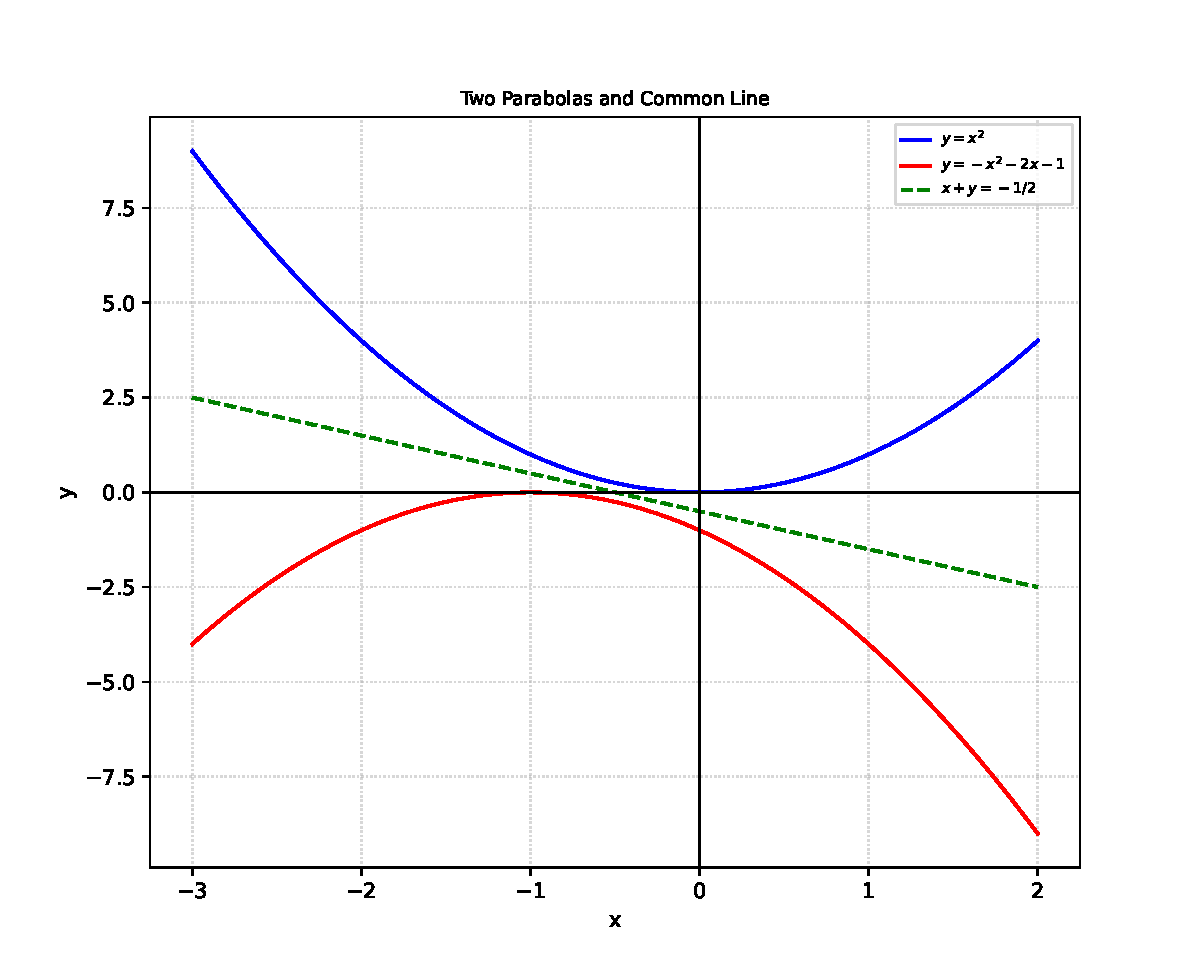
\includegraphics[width=0.7\columnwidth,keepaspectratio]{figs/q03.pdf}
\caption{The two parabolas and the line $x + y = -\frac{1}{2}$ from the pencil}
\end{figure}

\begin{lstlisting}[frame=single, basicstyle=\rmfamily, escapeinside={(*@}{@*)}]
(*@\makebox[\dimexpr\linewidth-2\fboxsep-2\fboxrule\relax][c]{codes/ce1q3/q03.py}@*)
\end{lstlisting}
\begin{lstlisting}[frame=single, basicstyle=\rmfamily, escapeinside={(*@}{@*)}]
(*@\makebox[\dimexpr\linewidth-2\fboxsep-2\fboxrule\relax][c]{codes/ce1q3/q03plot.py}@*)
\end{lstlisting}


% ----------------------------------------------------------- Q7
\item In the given figure, $\overline{PQ}$ is the diameter of a circle with center $O$. Two points $R$ and $S$ are chosen on the circle such that $\angle ROS = 80^\circ$. When $\overline{PR}$ and $\overline{QS}$ are extended, they meet at $T$. The value of $\angle RTS$ is \underline{\hspace{2cm}} \gate
\begin{multicols}{2}
\begin{enumerate}[label=\alph*), itemsep=0pt]
\item $40^\circ$
\item $50^\circ$
\item $60^\circ$
\item $80^\circ$
\end{enumerate}
\end{multicols}
\solution Let $O$ be the origin and the radius be $r$, with the diameter $PQ$ along the $x$-axis. Here $\vec{i}$ is the unit vector along the positive $x$-axis, and $\vec{w}_\theta$ is the unit vector that makes an angle $\theta$ with the positive $x$-axis, i.e. the point of the unit circle at angle $\theta$:
\begin{align}
\vec{i} \triangleq \myvec{1\\ 0},\quad \vec{w}_\theta \triangleq \myvec{\cos\theta\\ \sin\theta}
\end{align}
Since $PQ$ is a diameter, $\vec{P}$ and $\vec{Q}$ are opposite points on the $x$-axis. Let $\vec{R} = r\vec{w}_\alpha$ and $\vec{S} = r\vec{w}_\beta$ with $0 < \beta < \alpha < 180^\circ$. The points are listed in Table \ref{tab:q07}.
\begin{table}[H]
\centering
\begin{tabular}{|c|c|c|}
\hline
\textbf{Point} & \textbf{Vector} & \textbf{Description}\\ \hline
$O$ & $\vec{0}$ & centre\\ \hline
$P$ & $-r\vec{i}$ & end of diameter\\ \hline
$Q$ & $r\vec{i}$ & end of diameter\\ \hline
$R$ & $r\vec{w}_\alpha$ & on the circle\\ \hline
$S$ & $r\vec{w}_\beta$ & on the circle\\ \hline
\end{tabular}
\caption{Construction matrix of the points}
\label{tab:q07}
\end{table}
The construction matrix is
\begin{align}
\myvec{\vec{P} & \vec{Q} & \vec{R} & \vec{S}} = r\myvec{-\vec{i} & \vec{i} & \vec{w}_\alpha & \vec{w}_\beta}
\end{align}
From \eqref{eq:cosdiff},
\begin{align}
\cos\angle ROS = \vec{w}_\alpha^\top\vec{w}_\beta = \cos\brak{\alpha-\beta} \implies \alpha - \beta = 80^\circ
\end{align}
The direction vectors of the lines $PR$ and $QS$ are
\begin{align}
\vec{R} - \vec{P} &= r\myvec{1+\cos\alpha\\ \sin\alpha} = 2r\cos\frac{\alpha}{2}\myvec{\cos\frac{\alpha}{2}\\ \sin\frac{\alpha}{2}}\\
\vec{S} - \vec{Q} &= r\myvec{\cos\beta - 1\\ \sin\beta} = 2r\sin\frac{\beta}{2}\myvec{-\sin\frac{\beta}{2}\\ \cos\frac{\beta}{2}}
\end{align}
The point $T$ lies beyond $R$ on $PR$ and beyond $S$ on $QS$. Hence $\overrightarrow{TR}$ is along $\vec{P} - \vec{R}$ and $\overrightarrow{TS}$ is along $\vec{Q} - \vec{S}$. Using \eqref{eq:angle},
\begin{align}
\cos\angle RTS &= \myvec{\cos\frac{\alpha}{2} & \sin\frac{\alpha}{2}}\myvec{-\sin\frac{\beta}{2}\\ \cos\frac{\beta}{2}}\\
&= \sin\frac{\alpha}{2}\cos\frac{\beta}{2} - \cos\frac{\alpha}{2}\sin\frac{\beta}{2} = \sin\frac{\alpha-\beta}{2}\\
&= \sin 40^\circ = \cos 50^\circ\\
\implies \angle RTS &= 50^\circ
\end{align}
For a numerical check, take $r = 1$, $\alpha = 130^\circ$, $\beta = 50^\circ$. From \eqref{eq:lineint},
\begin{align}
\myvec{\vec{R}-\vec{P} & -\brak{\vec{S}-\vec{Q}}}\myvec{\kappa_1\\ \kappa_2} = \vec{Q} - \vec{P} \implies \vec{T} = \myvec{0\\ 2.1445}
\end{align}
and \eqref{eq:angle} gives $\angle RTS = 50^\circ$.
\begin{figure}[H]
\centering
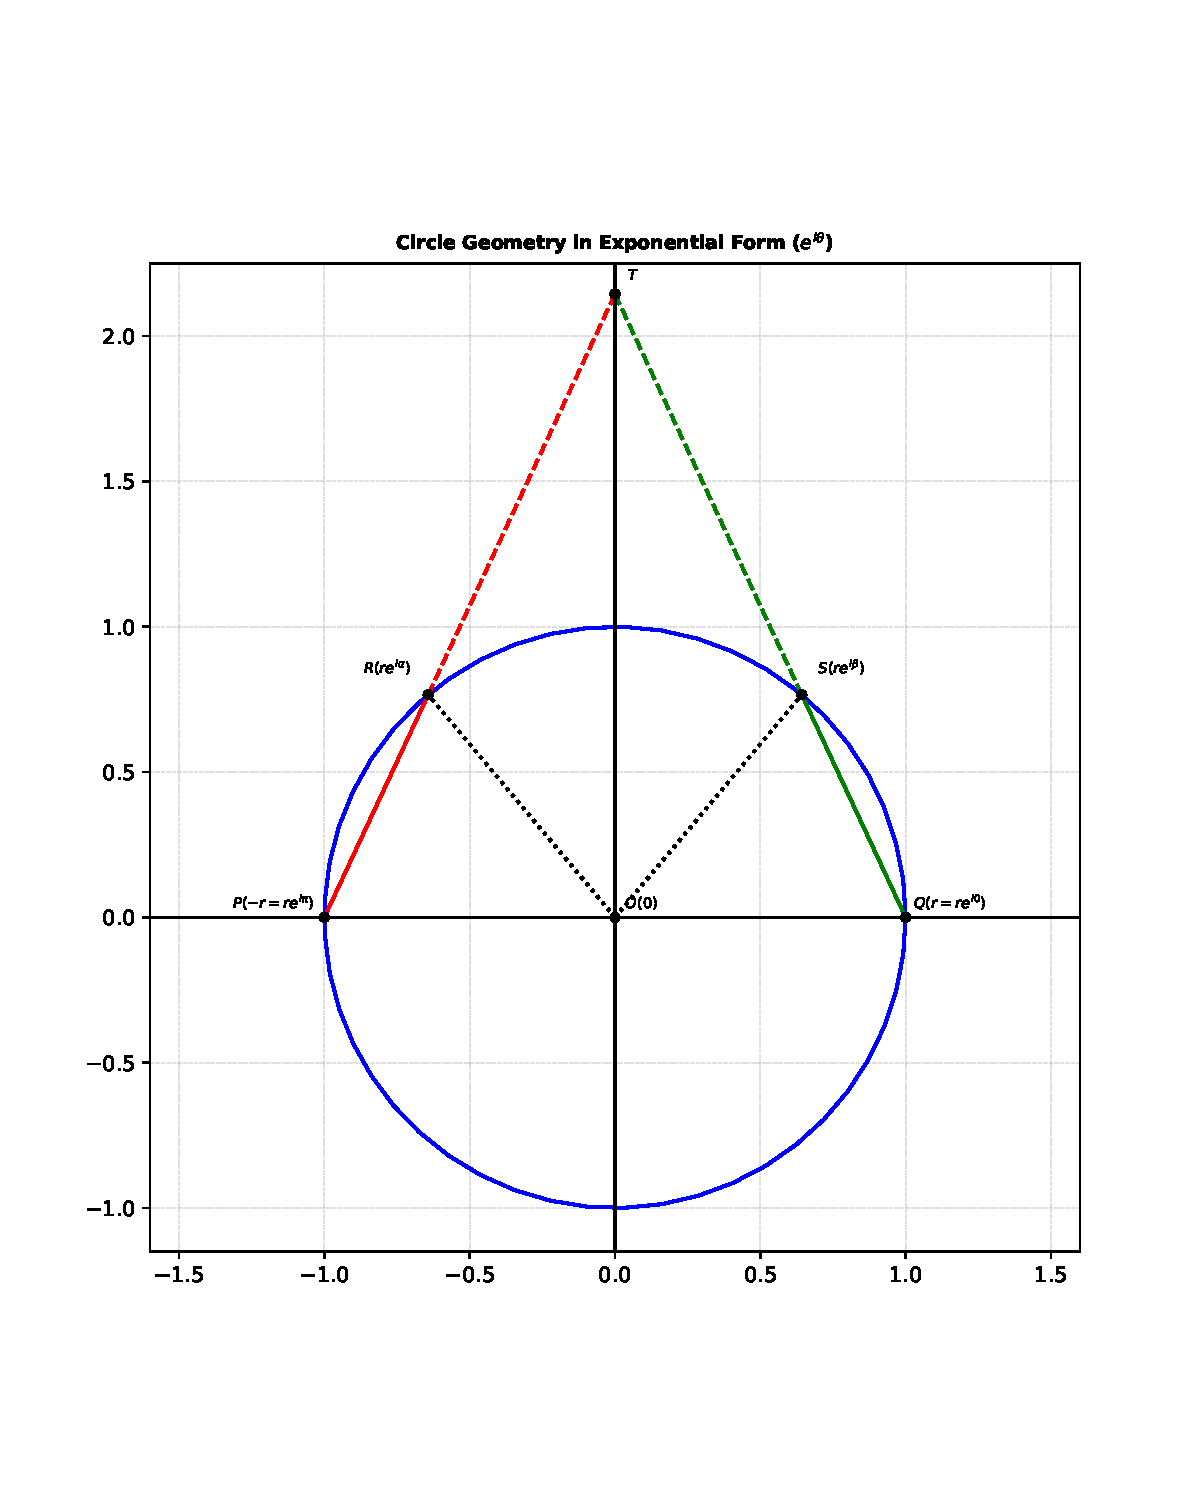
\includegraphics[width=0.7\columnwidth,keepaspectratio]{figs/q07.pdf}
\caption{Circle with diameter $PQ$, $\angle ROS = 80^\circ$ and $\angle RTS = 50^\circ$}
\end{figure}

\begin{lstlisting}[frame=single, basicstyle=\rmfamily, escapeinside={(*@}{@*)}]
(*@\makebox[\dimexpr\linewidth-2\fboxsep-2\fboxrule\relax][c]{codes/ce1q7/q07.py}@*)
\end{lstlisting}
\begin{lstlisting}[frame=single, basicstyle=\rmfamily, escapeinside={(*@}{@*)}]
(*@\makebox[\dimexpr\linewidth-2\fboxsep-2\fboxrule\relax][c]{codes/ce1q7/q07plot.py}@*)
\end{lstlisting}







%------------------------------------------------------------Q9

\item Consider a linear arrangement of seven bulbs, each of which can be in the ON or OFF states. The initial configuration of the bulbs is shown in the figure. In every Step, the states of the bulbs are changed based on the following rules: Any OFF bulb with exactly one ON neighbor at the end of the previous Step is turned ON. Any ON bulb with both neighbors ON at the end of the previous Step is turned OFF. The state of any bulb not meeting the conditions above is left unchanged. The state of bulbs at the end of Step 1 and Step 2 are also shown in the figure. The number of bulbs which are ON at the end of Step 8 is \hfill (GATE CE 2026)

\begin{multicols}{2}
\begin{enumerate}[(a)]
    \item 5
    \item 4
    \item 3
    \item 0
\end{enumerate}
\end{multicols}

% Helper macro: \bulb{x}{y}{fill_color}
\newcommand{\bulb}[3]{
  \draw[fill=#3, thick] (#1,#2) circle (0.16);
  \draw[fill=white, thin] (#1-0.05, #2-0.24) rectangle (#1+0.05, #2-0.15);
}

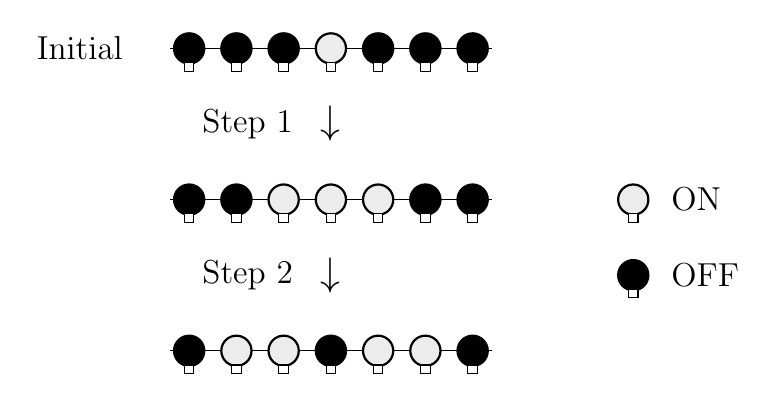
\begin{tikzpicture}[scale=1.2]

  % --- Row 1: Initial ---
  \node[font=\large, anchor=east] at (0.4, 2.8) {Initial};
  \draw[thin] (0.8, 2.8) -- (4.2, 2.8);
  
  \bulb{1.0}{2.8}{black}
  \bulb{1.5}{2.8}{black}
  \bulb{2.0}{2.8}{black}
  \bulb{2.5}{2.8}{gray!15}
  \bulb{3.0}{2.8}{black}
  \bulb{3.5}{2.8}{black}
  \bulb{4.0}{2.8}{black}

  % --- Step 1 Arrow ---
  \node[font=\large, anchor=east] at (2.2, 2.0) {Step 1};
  \node[font=\Large] at (2.5, 2.0) {$\downarrow$};

  % --- Row 2: Step 1 ---
  \draw[thin] (0.8, 1.2) -- (4.2, 1.2);
  
  \bulb{1.0}{1.2}{black}
  \bulb{1.5}{1.2}{black}
  \bulb{2.0}{1.2}{gray!15}
  \bulb{2.5}{1.2}{gray!15}
  \bulb{3.0}{1.2}{gray!15}
  \bulb{3.5}{1.2}{black}
  \bulb{4.0}{1.2}{black}

  % --- Step 2 Arrow ---
  \node[font=\large, anchor=east] at (2.2, 0.4) {Step 2};
  \node[font=\Large] at (2.5, 0.4) {$\downarrow$};

  % --- Row 3: Step 2 ---
  \draw[thin] (0.8, -0.4) -- (4.2, -0.4);
  
  \bulb{1.0}{-0.4}{black}
  \bulb{1.5}{-0.4}{gray!15}
  \bulb{2.0}{-0.4}{gray!15}
  \bulb{2.5}{-0.4}{black}
  \bulb{3.0}{-0.4}{gray!15}
  \bulb{3.5}{-0.4}{gray!15}
  \bulb{4.0}{-0.4}{black}

  % --- Legend ---
  \bulb{5.7}{1.2}{gray!15}
  \node[font=\large, anchor=west] at (6.0, 1.2) {ON};

  \bulb{5.7}{0.4}{black}
  \node[font=\large, anchor=west] at (6.0, 0.4) {OFF};

\end{tikzpicture}

\solution Let $x_k \in \{0,1\}^7$ be the state vector after Step $k$ and $s_k = Ax_k$, where
\[
A = \begin{pmatrix}
0 & 1 & 0 & 0 & 0 & 0 & 0 \\
1 & 0 & 1 & 0 & 0 & 0 & 0 \\
0 & 1 & 0 & 1 & 0 & 0 & 0 \\
0 & 0 & 1 & 0 & 1 & 0 & 0 \\
0 & 0 & 0 & 1 & 0 & 1 & 0 \\
0 & 0 & 0 & 0 & 1 & 0 & 1 \\
0 & 0 & 0 & 0 & 0 & 1 & 0
\end{pmatrix}
\]
The rules give the update:
\[
x_{k+1} = x_k + (1 - x_k) \odot [s_k = 1] - x_k \odot [s_k = 2]
\]
where $\odot$ is the element-wise product and $[\cdot]$ is 1 when the condition holds. The initial configuration has only the middle bulb ON:
\[
x_0 = \begin{pmatrix} 0 & 0 & 0 & 1 & 0 & 0 & 0 \end{pmatrix}^\top, \quad s_0 = \begin{pmatrix} 0 & 0 & 1 & 0 & 1 & 0 & 0 \end{pmatrix}^\top
\]
\[
x_1 = \begin{pmatrix} 0 & 0 & 1 & 1 & 1 & 0 & 0 \end{pmatrix}^\top, \quad s_1 = \begin{pmatrix} 0 & 1 & 1 & 2 & 1 & 1 & 0 \end{pmatrix}^\top
\]
\[
x_2 = \begin{pmatrix} 0 & 1 & 1 & 0 & 1 & 1 & 0 \end{pmatrix}^\top, \quad s_2 = \begin{pmatrix} 1 & 1 & 2 & 1 & 1 & 1 & 1 \end{pmatrix}^\top
\]
\[
x_3 = \begin{pmatrix} 1 & 1 & 1 & 0 & 1 & 1 & 1 \end{pmatrix}^\top, \quad s_3 = \begin{pmatrix} 1 & 2 & 1 & 2 & 1 & 2 & 1 \end{pmatrix}^\top
\]
\[
x_4 = \begin{pmatrix} 1 & 0 & 1 & 0 & 1 & 0 & 1 \end{pmatrix}^\top, \quad s_4 = \begin{pmatrix} 0 & 2 & 0 & 2 & 0 & 2 & 0 \end{pmatrix}^\top
\]
$x_1$ and $x_2$ agree with Step 1 and Step 2 in the figure. In $x_4$, every OFF bulb has two ON neighbours and every ON bulb has none, so:
\[
x_5 = x_4 \Rightarrow x_8 = x_4 = \begin{pmatrix} 1 & 0 & 1 & 0 & 1 & 0 & 1 \end{pmatrix}^\top
\]
The number of bulbs which are ON at the end of Step 8 is:
\[
1^\top x_8 = 4
\]

\begin{lstlisting}[frame=single, basicstyle=\rmfamily, escapeinside={(*@}{@*)}]
(*@\makebox[\dimexpr\linewidth-2\fboxsep-2\fboxrule\relax][c]{codes/ce1q9/q09.py}@*)
\end{lstlisting}
%-------------------------------------------------------------Q10

\item $P$ and $Q$ are two positive integers such that $P^2 = Q^2 + 13$. The product of the numbers $P$ and $Q$ is \underline{\hspace{2cm}} \hfill (GATE CE 2026)
\begin{multicol}{2}
\begin{enumerate}[label=\alph*)]
        \item 13
        \item 26
        \item 39
        \item 42
\end{enumerate}
\end{multicol}

\solution The given equation can be written as
\begin{equation}
    P^2 - Q^2 = (P - Q)(P + Q) = 13 \tag{1.2.4.1}
\end{equation}
    Since 13 is prime and $0 < P - Q < P + Q$,
\begin{equation}
    P - Q = 1, \quad P + Q = 13 \tag{1.2.4.2}
\end{equation}

    Expressing in the matrix form \eqref{eq:axb} :
\begin{equation}
\begin{pmatrix} 1 & -1 \\ 1 & 1 \end{pmatrix} \begin{pmatrix} P \\ Q \end{pmatrix} = \begin{pmatrix} 1 \\ 13 \end{pmatrix} \tag{1.2.4.3}
\end{equation}

    Applying $R_2 \rightarrow R_2 - R_1$ on the augmented matrix:
\begin{equation}
\begin{pmatrix} 1 & -1 & 1 \\ 1 & 1 & 13 \end{pmatrix} \xrightarrow{R_2 \rightarrow R_2 - R_1} \begin{pmatrix} 1 & -1 & 1 \\ 0 & 2 & 12 \end{pmatrix} \implies Q = 6,\ P = 7 \tag{1.2.4.4}
\end{equation}

    Therefore,
\begin{equation}
    PQ = 7 \times 6 = 42 \tag{1.2.4.5}
\end{equation}
\end{enumerate}



% ----------------------------------------------------------- Q11 (1.1.15)
\item Matrix $\vec{P}$ is given as
\begin{align}
\vec{P} = \myvec{1 & 0 & 1\\ 0 & 1 & 0\\ 1 & 0 & 1}
\end{align}
The TRUE option is \gate
\begin{multicols}{2}
\begin{enumerate}[label=\alph*), itemsep=0pt]
\item Trace of $\vec{P}$ is equal to the sum of the Eigen values of $\vec{P}$.
\item $\vec{P}^\top\vec{P}$ is an identity matrix.
\item $\vec{P}$ is a skew-symmetric matrix.
\item Absolute magnitude of each Eigen value is 1.
\end{enumerate}
\end{multicols}
\solution From \eqref{eq:charpoly}, expanding along the second row,
\begin{align}
\abs{\lambda\vec{I} - \vec{P}} &= \mydet{\lambda-1 & 0 & -1\\ 0 & \lambda-1 & 0\\ -1 & 0 & \lambda-1}\\
&= \brak{\lambda-1}\sbrak{\brak{\lambda-1}^2 - 1}\\
&= \lambda\brak{\lambda-1}\brak{\lambda-2} = 0\\
\implies \lambda_1 &= 0,\ \lambda_2 = 1,\ \lambda_3 = 2
\end{align}
From \eqref{eq:trace}:
\begin{align}
\text{tr}\brak{\vec{P}} = 1+1+1 = 3 = \lambda_1 + \lambda_2 + \lambda_3
\end{align}
so option (A) is true. The remaining options are false since
\begin{align}
\vec{P}^\top\vec{P} &= \myvec{2 & 0 & 2\\ 0 & 1 & 0\\ 2 & 0 & 2} \neq \vec{I}\\
\vec{P}^\top &= \vec{P} \neq -\vec{P}\\
\abs{\lambda_1} &= 0 \neq 1
\end{align}
\begin{lstlisting}[frame=single, basicstyle=\rmfamily, escapeinside={(*@}{@*)}]
(*@\makebox[\dimexpr\linewidth-2\fboxsep-2\fboxrule\relax][c]{codes/ce1q11/q11.py}@*)
\end{lstlisting}

% ----------------------------------------------------------- Q12
\item Given:
\begin{align}
\myvec{1 & 1 & 1\\ 1 & 0 & 2}\myvec{x_1\\ x_2\\ x_3} = \myvec{0\\ 0}
\end{align}
The above system of equations represents a \gate
\begin{multicols}{2}
\begin{enumerate}[label=\alph*), itemsep=0pt]
\item plane
\item line
\item volume
\item point
\end{enumerate}
\end{multicols}
\solution The augmented matrix is reduced as
\begin{align}
\myvec{1 & 1 & 1 & 0\\ 1 & 0 & 2 & 0} \xrightarrow{R_2\to R_2 - R_1} \myvec{1 & 1 & 1 & 0\\ 0 & -1 & 1 & 0}
\end{align}
Thus,
\begin{align}
\text{rank}\brak{\vec{A}} = \text{rank}\brak{{\vec{A}\mid\vec{b}}} = 2 < n = 3
\end{align}
From \eqref{eq:rc}, the system is consistent with $n - r = 1$ free variable. From \eqref{eq:cross}, the solution is
\begin{align}
\vec{x} = \kappa\brak{\myvec{1\\ 1\\ 1}\times\myvec{1\\ 0\\ 2}} = \kappa\myvec{2\\ -1\\ -1},\quad \kappa\in\mathbb{R}
\end{align}
which is a line through the origin (the intersection of two planes).

\begin{figure}[H]
\centering
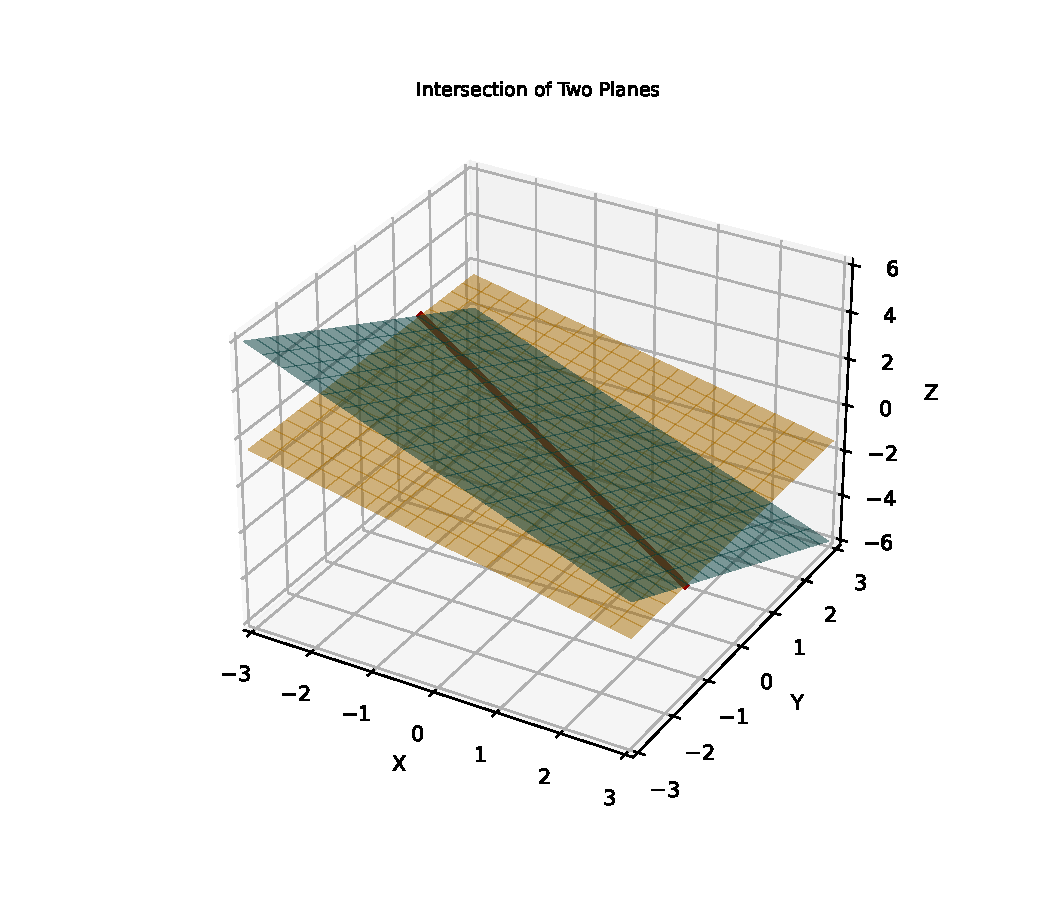
\includegraphics[width=0.7\columnwidth,keepaspectratio]{figs/q12.pdf}
\caption{The two planes and their line of intersection}
\end{figure}
\begin{lstlisting}[frame=single, basicstyle=\rmfamily, escapeinside={(*@}{@*)}]
(*@\makebox[\dimexpr\linewidth-2\fboxsep-2\fboxrule\relax][c]{codes/ce1q12/q12.py}@*)
\end{lstlisting}
\begin{lstlisting}[frame=single, basicstyle=\rmfamily, escapeinside={(*@}{@*)}]
(*@\makebox[\dimexpr\linewidth-2\fboxsep-2\fboxrule\relax][c]{codes/ce1q12/q12plot.py}@*)
\end{lstlisting}

% ----------------------------------------------------------- Q26
\item Bag I contains 4 white and 6 black balls. Bag II contains 4 white and 3 black balls. One ball is drawn at random from any one of the two bags and it is found to be a black ball. The probability that the black ball was drawn from Bag I is \underline{\hspace{2cm}} (rounded off to two decimal places). \gate

\solution Let $B_1$, $B_2$ denote choosing Bag I, Bag II and $E$ the event of drawing a black ball. The prior and likelihood vectors are
\begin{align}
\vec{\pi} = \myvec{\frac{1}{2}\\ \frac{1}{2}},\quad \vec{l} = \myvec{\frac{6}{10}\\ \frac{3}{7}}
\end{align}
From \eqref{eq:total},
\begin{align}
\pr{E} = \vec{\pi}^\top\vec{l} = \frac{1}{2}\brak{\frac{3}{5} + \frac{3}{7}} = \frac{18}{35}
\end{align}
From \eqref{eq:bayes},
\begin{align}
\pr{B_1\mid E} = \frac{\frac{1}{2}\times\frac{3}{5}}{\frac{18}{35}} = \frac{3}{10}\times\frac{35}{18} = \frac{7}{12} \approx 0.58
\end{align}
\begin{lstlisting}[frame=single, basicstyle=\rmfamily, escapeinside={(*@}{@*)}]
(*@\makebox[\dimexpr\linewidth-2\fboxsep-2\fboxrule\relax][c]{codes/ce1q26/q26.py}@*)
\end{lstlisting}

% ----------------------------------------------------------- Q27
\item A matrix is given as:
\begin{align}
\myvec{9 & 15\\ 15 & 50}
\end{align}

\solution A symmetric positive definite matrix $A \in \mathbb{R}^{2 \times 2}$ given as
\[
    A = \begin{pmatrix} 9 & 15 \\ 15 & 50 \end{pmatrix}
\]
can be factored using standard LU decomposition into $A = L_{\text{LU}} U$ with a unit lower triangular matrix $L_{\text{LU}}$:
\begin{equation}
    \begin{pmatrix} 1 & 0 \\ l_{21} & 1 \end{pmatrix} \begin{pmatrix} u_{11} & u_{12} \\ 0 & u_{22} \end{pmatrix} = \begin{pmatrix} u_{11} & u_{12} \\ l_{21}u_{11} & l_{21}u_{12} + u_{22} \end{pmatrix} = \begin{pmatrix} 9 & 15 \\ 15 & 50 \end{pmatrix} \label{eq:lu_system}
\end{equation}
Equating entries yields $u_{11} = 9$, $u_{12} = 15$, $l_{21} = 15/9 = 5/3$, and $u_{22} = 50 - (5/3)(15) = 25$. This gives:
\begin{equation}
    L_{\text{LU}} = \begin{pmatrix} 1 & 0 \\ \frac{5}{3} & 1 \end{pmatrix}, \quad U = \begin{pmatrix} 9 & 15 \\ 0 & 25 \end{pmatrix} \label{eq:lu_result}
\end{equation}
Factoring out the diagonal matrix $D = \text{diag}(9, 25)$ transforms the LU decomposition into $A = L_{\text{LU}} D L_{\text{LU}}^\top$:
\begin{equation}
    A = \begin{pmatrix} 1 & 0 \\ \frac{5}{3} & 1 \end{pmatrix} \begin{pmatrix} 9 & 0 \\ 0 & 25 \end{pmatrix} \begin{pmatrix} 1 & \frac{5}{3} \\ 0 & 1 \end{pmatrix} \label{eq:ldl_result}
\end{equation}
By absorbing $D^{1/2} = \text{diag}(\sqrt{9}, \sqrt{25}) = \text{diag}(3, 5)$ into $L_{\text{LU}}$, the Cholesky factor $L$ for $A = LL^\top$ is derived:
\begin{equation}
    L = L_{\text{LU}} D^{1/2} = \begin{pmatrix} 1 & 0 \\ \frac{5}{3} & 1 \end{pmatrix} \begin{pmatrix} 3 & 0 \\ 0 & 5 \end{pmatrix} = \begin{pmatrix} 3 & 0 \\ 5 & 5 \end{pmatrix} \label{eq:cholesky_from_lu}
\end{equation}

Alternatively, using the general Cholesky algorithm directly, $A = LL^\top$ computes $l_{ij}$ for $1 \le j \le i \le n$ via:
\begin{equation}
    l_{jj} = \sqrt{a_{jj} - \sum_{k=1}^{j-1} l_{jk}^2} \label{eq:cholesky_diag}
\end{equation}
\begin{equation}
    l_{ij} = \frac{1}{l_{jj}} \left( a_{ij} - \sum_{k=1}^{j-1} l_{ik} l_{jk} \right), \quad \text{for } i > j \label{eq:cholesky_offdiag}
\end{equation}
Evaluating Equation~\eqref{eq:cholesky_diag} for $j = 1$ gives:
\begin{equation}
    l_{11} = \sqrt{a_{11}} = \sqrt{9} = 3 \label{eq:step_l11}
\end{equation}
Evaluating Equation~\eqref{eq:cholesky_offdiag} for $i = 2, j = 1$ gives:
\begin{equation}
    l_{21} = \frac{a_{21}}{l_{11}} = \frac{15}{3} = 5 \label{eq:step_l21}
\end{equation}
Evaluating Equation~\eqref{eq:cholesky_diag} for $j = 2$ gives:
\begin{equation}
    l_{22} = \sqrt{a_{22} - l_{21}^2} = \sqrt{50 - 5^2} = \sqrt{25} = 5 \label{eq:step_l22}
\end{equation}
Both approaches confirm that the Cholesky factor matrix and diagonal value are:
\begin{equation}
    L = \begin{pmatrix} 3 & 0 \\ 5 & 5 \end{pmatrix}, \quad |l_{22}| = 5 \label{eq:final_answer}
\end{equation}
\begin{lstlisting}[frame=single, basicstyle=\rmfamily, escapeinside={(*@}{@*)}]
(*@\makebox[\dimexpr\linewidth-2\fboxsep-2\fboxrule\relax][c]{codes/ce1q27/q27.py}@*)
\end{lstlisting}

% ----------------------------------------------------------- Q28
\item It is given that $x$ and $y$ are integers in the following equation:
\begin{align}
\brak{x + y - 7}^2 + \brak{y + 3x - 13}^2 = 0
\end{align}


The value of $\brak{x^3 + y^3}$ is \underline{\hspace{2cm}} (in integer). \gate

\solution Let
\begin{align}
\vec{A} = \myvec{1 & 1\\ 3 & 1},\quad \vec{b} = \myvec{7\\ 13},\quad \vec{x} = \myvec{x\\ y}
\end{align}
The given equation is
\begin{align}
\norm{\vec{A}\vec{x} - \vec{b}}^2 = 0
\end{align}
From \eqref{eq:zeronorm},
\begin{align}
\vec{A}\vec{x} = \vec{b}
\end{align}
Reducing the augmented matrix:
\begin{align}
\myvec{1 & 1 & 7\\ 3 & 1 & 13} \xrightarrow{R_2\to R_2 - 3R_1} \myvec{1 & 1 & 7\\ 0 & -2 & -8} \implies y = 4,\ x = 3
\end{align}
Therefore,
\begin{align}
x^3 + y^3 = 27 + 64 = 91
\end{align}
\begin{lstlisting}[frame=single, basicstyle=\rmfamily, escapeinside={(*@}{@*)}]
(*@\makebox[\dimexpr\linewidth-2\fboxsep-2\fboxrule\relax][c]{codes/ce1q28/q28.py}@*)
\end{lstlisting}
\begin{lstlisting}[frame=single, basicstyle=\rmfamily, escapeinside={(*@}{@*)}]
(*@\makebox[\dimexpr\linewidth-2\fboxsep-2\fboxrule\relax][c]{codes/ce1q28/q28plot.py}@*)
\end{lstlisting}

% ----------------------------------------------------------- Q36
\item Let $f\brak{x}$ be a continuous function defined in $\sbrak{0,2}\to\mathbb{R}$ and satisfying the equation
\begin{align}
\int_0^2 f\brak{x}\sbrak{x - f\brak{x}}dx = \frac{2}{3}
\end{align}
The value of $f\brak{1}$ is \gate
\begin{multicols}{2}
\begin{enumerate}[label=\alph*), itemsep=0pt]
\item 1
\item 2
\item $\frac{1}{2}$
\item 0
\end{enumerate}
\end{multicols}
\solution Using \eqref{eq:cts} with $a = x$ and $b = f\brak{x}$:
\begin{align}
f\brak{x}\sbrak{x - f\brak{x}} = \frac{x^2}{4} - \brak{f\brak{x} - \frac{x}{2}}^2
\end{align}
Integrating over $\sbrak{0,2}$:
\begin{align}
\int_0^2 f\brak{x}\sbrak{x - f\brak{x}}dx &= \int_0^2\frac{x^2}{4}dx - \int_0^2\brak{f\brak{x} - \frac{x}{2}}^2dx\\
&= \frac{2}{3} - \int_0^2\brak{f\brak{x} - \frac{x}{2}}^2dx
\end{align}
Equating with the given value,
\begin{align}
\int_0^2\brak{f\brak{x} - \frac{x}{2}}^2dx = 0
\end{align}
Since the integrand is continuous and non-negative,
\begin{align}
f\brak{x} = \frac{x}{2} \implies f\brak{1} = \frac{1}{2}
\end{align}

\begin{figure}[H]
\centering
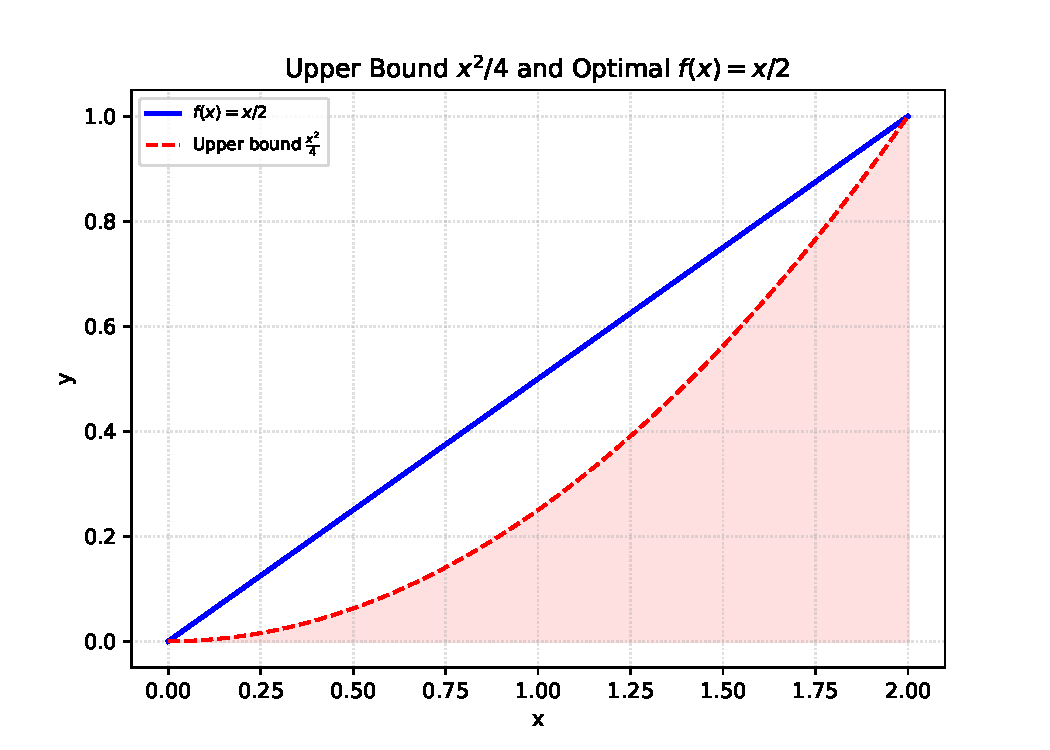
\includegraphics[width=0.7\columnwidth,keepaspectratio]{figs/q36.pdf}
\caption{The integrand attains its upper bound $\frac{x^2}{4}$ only for $f\brak{x} = \frac{x}{2}$}
\end{figure}
\begin{lstlisting}[frame=single, basicstyle=\rmfamily, escapeinside={(*@}{@*)}]
(*@\makebox[\dimexpr\linewidth-2\fboxsep-2\fboxrule\relax][c]{codes/ce1q36/q36.py}@*)
\end{lstlisting}
\begin{lstlisting}[frame=single, basicstyle=\rmfamily, escapeinside={(*@}{@*)}]
(*@\makebox[\dimexpr\linewidth-2\fboxsep-2\fboxrule\relax][c]{codes/ce1q36/q36plot.py}@*)
\end{lstlisting}

% ----------------------------------------------------------- Q37
\item An ordinary differential equation is given below.
\begin{align}
x^2\frac{d^2y}{dx^2} = 6y
\end{align}
Considering $a$ and $b$ as arbitrary constants, the general solution of the equation is \gate
\begin{multicols}{2}
\begin{enumerate}[label=\alph*), itemsep=0pt]
\item $y\brak{x} = ax^3 + \frac{b}{x^2}$
\item $y\brak{x} = ax^2 + \frac{b}{x^3}$
\item $y\brak{x} = ax^2 + b\ln x$
\item $y\brak{x} = ax^3 + b\ln x$
\end{enumerate}
\end{multicols}
\solution Let $x = e^t$ $\brak{x > 0}$. Then
\begin{align}
x\frac{dy}{dx} = \frac{dy}{dt},\quad x^2\frac{d^2y}{dx^2} = \frac{d^2y}{dt^2} - \frac{dy}{dt}
\end{align}
and the equation becomes
\begin{align}
y'' - y' - 6y = 0
\label{eq:q37t}
\end{align}
Taking the Laplace transform using \eqref{eq:lap1} and \eqref{eq:lap2}:
\begin{align}
s^2Y\brak{s} - sy\brak{0} - y'\brak{0} - \sbrak{sY\brak{s} - y\brak{0}} - 6Y\brak{s} &= 0\\
Y\brak{s} = \frac{\brak{s-1}y\brak{0} + y'\brak{0}}{s^2 - s - 6} &= \frac{\brak{s-1}y\brak{0} + y'\brak{0}}{\brak{s-3}\brak{s+2}}
\end{align}
Decomposing into partial fractions and using \eqref{eq:lapexp},
\begin{align}
Y\brak{s} = \frac{a}{s-3} + \frac{b}{s+2} \implies y\brak{t} = ae^{3t} + be^{-2t}
\end{align}
Substituting $e^t = x$:
\begin{align}
y\brak{x} = ax^3 + \frac{b}{x^2}
\end{align}

\begin{lstlisting}[frame=single, basicstyle=\rmfamily, escapeinside={(*@}{@*)}]
(*@\makebox[\dimexpr\linewidth-2\fboxsep-2\fboxrule\relax][c]{codes/ce1q37/q37.py}@*)
\end{lstlisting}

% ----------------------------------------------------------- Q38
\item A plane truss consists of two linearly elastic, homogeneous, identical members, namely $PQ$ and $QR$. Both members have length $\brak{L}$, cross-sectional area $\brak{A}$, and modulus of elasticity $\brak{E}$. The members are inclined at $45^\circ$ as shown in the figure. The truss has hinge supports at $P$ and $R$. The translational degrees-of-freedom ($u$ and $v$) are shown at joint $Q$.


\begin{center}
\begin{tikzpicture}[scale=1.2]

    % --- Coordinates ---
    \coordinate (P) at (0, 0);
    \coordinate (Q) at (3, 2.8);
    \coordinate (R) at (6, 0);

    % --- Thin Horizontal Reference Line ---
    \draw[thin, gray!70] (P) -- (R);

    % --- Support at P ---
    \fill[gray!50] (P) -- (-0.4, -0.5) -- (0.4, -0.5) -- cycle;
    \draw[line width=1pt] (P) -- (-0.4, -0.5) -- (0.4, -0.5) -- cycle;
    \draw[line width=1pt] (-0.6, -0.5) -- (0.6, -0.5);
    \fill[pattern=north east lines] (-0.6, -0.8) rectangle (0.6, -0.5);

    % --- Support at R ---
    \fill[gray!50] (R) -- (5.6, -0.5) -- (6.4, -0.5) -- cycle;
    \draw[line width=1pt] (R) -- (5.6, -0.5) -- (6.4, -0.5) -- cycle;
    \draw[line width=1pt] (5.4, -0.5) -- (6.6, -0.5);
    \fill[pattern=north east lines] (5.4, -0.8) rectangle (6.6, -0.5);

    % --- Truss Members ---
    \draw[line width=1.8pt] (P) -- (Q);
    \draw[line width=1.8pt] (Q) -- (R);

    % --- Member Properties (A, E, L) ---
    \node[above left, font=\large\itshape] at (1.5, 1.4) {$A, E, L$};
    \node[above right, font=\large\itshape] at (4.5, 1.4) {$A, E, L$};

    % --- Joint Labels ---
    \node[left, font=\large\bfseries] at (-0.1, 0.15) {P};
    \node[right, font=\large\bfseries] at (6.1, 0.15) {R};
    \node[left, font=\large\bfseries] at (Q) {Q\ };

    % --- Displacement / Coordinate Axes at Q ---
    \draw[->, >=Stealth, line width=1.2pt] (Q) -- ++(1.4, 0) node[right, font=\large\itshape] {$u$};
    \draw[->, >=Stealth, line width=1.2pt] (Q) -- ++(0, 1.3) node[above, font=\large\itshape] {$v$};

    % --- Angle Arcs & Labels ---
    % Angle at P
    \draw[line width=0.8pt] (0.8, 0) arc (0:43:0.8);
    \node at (1.35, 0.35) {\large $45^\circ$};

    % Angle at R
    \draw[line width=0.8pt] (5.2, 0) arc (180:137:0.8);
    \node at (4.65, 0.35) {\large $45^\circ$};

    % --- Caption / Note ---
    \node[font=\large\bfseries] at (3, -1.3) {(Figure not to scale)};

\end{tikzpicture}
\end{center}

After application of the boundary conditions, the stiffness matrix of the truss becomes: \gate
\begin{multicols}{2}
\begin{enumerate}[label=\alph*), itemsep=0pt]
\item $\frac{AE}{L}\myvec{1 & 1\\ 1 & 1}$
\item $\frac{AE}{L}\myvec{1 & 0.5\\ 0.5 & 1}$
\item $\frac{AE}{L}\myvec{1 & 0\\ 0 & 1}$
\item $\frac{AE}{L}\myvec{1 & -1\\ -1 & 1}$
\end{enumerate}
\end{multicols}
\solution The unit direction vectors of the members are
\begin{align}
\vec{m}_{PQ} = \frac{1}{\sqrt{2}}\myvec{1\\ 1},\quad \vec{m}_{QR} = \frac{1}{\sqrt{2}}\myvec{1\\ -1}
\end{align}
From \eqref{eq:kbar},
\begin{align}
\vec{k}_{PQ} &= \frac{AE}{L}\vec{m}_{PQ}\vec{m}_{PQ}^\top = \frac{AE}{L}\myvec{0.5 & 0.5\\ 0.5 & 0.5}\\
\vec{k}_{QR} &= \frac{AE}{L}\vec{m}_{QR}\vec{m}_{QR}^\top = \frac{AE}{L}\myvec{0.5 & -0.5\\ -0.5 & 0.5}
\end{align}
After deleting the restrained degrees of freedom at $P$ and $R$, only the $\brak{u,v}$ block at $Q$ receives contributions from both members:
\begin{align}
\vec{K} = \vec{k}_{PQ} + \vec{k}_{QR} = \frac{AE}{L}\myvec{1 & 0\\ 0 & 1}
\end{align}

\begin{figure}[H]
\centering
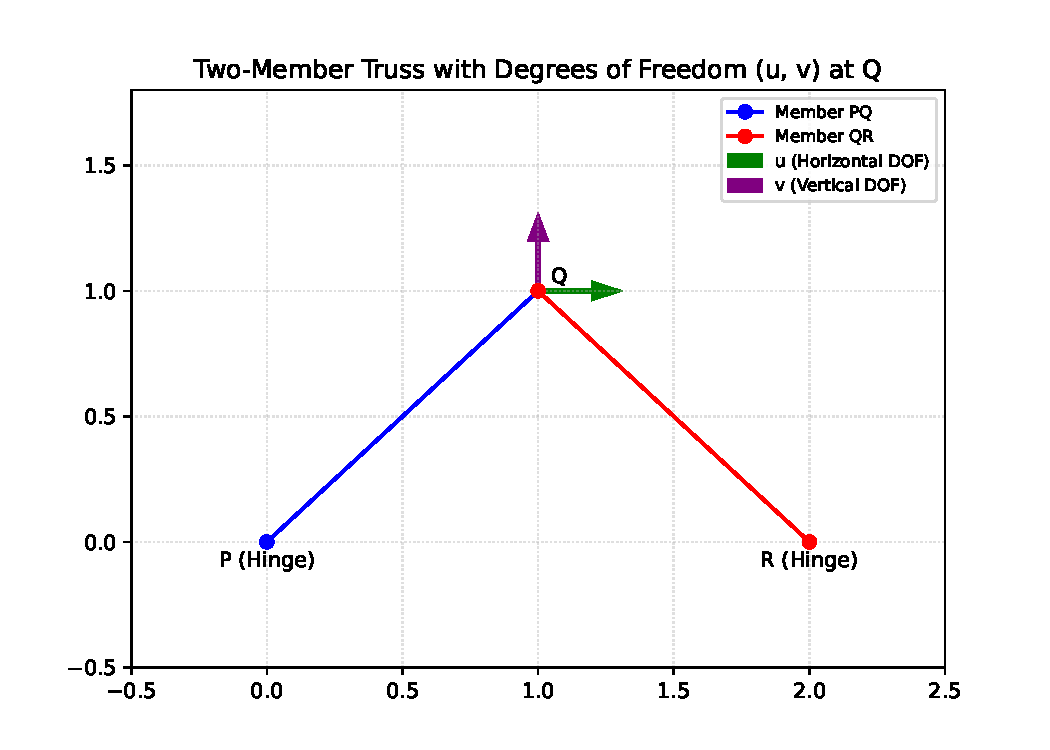
\includegraphics[width=0.7\columnwidth,keepaspectratio]{figs/q38.pdf}
\caption{Two-member truss with degrees of freedom $u$, $v$ at $Q$}
\end{figure}
\begin{lstlisting}[frame=single, basicstyle=\rmfamily, escapeinside={(*@}{@*)}]
(*@\makebox[\dimexpr\linewidth-2\fboxsep-2\fboxrule\relax][c]{codes/ce1q38/q38.py}@*)
\end{lstlisting}
\begin{lstlisting}[frame=single, basicstyle=\rmfamily, escapeinside={(*@}{@*)}]
(*@\makebox[\dimexpr\linewidth-2\fboxsep-2\fboxrule\relax][c]{codes/ce1q38/q38plot.py}@*)
\end{lstlisting}

% ----------------------------------------------------------- Q39
\item The plane frame has a hinge and a roller support, and is loaded as shown in the figure. Both the columns have same height.

What is the absolute value of the maximum bending moment (in kN-m) in the frame? \hfill (GATE CE 2026)

\begin{multicols}{2}
\begin{enumerate}[label=\alph*)]
    \item 165
    \item 150
    \item 240
    \item 195
\end{enumerate}
\end{multicols}
\begin{center}
\begin{tikzpicture}[scale=1.2]

    % --- Frame Coordinates ---
    \coordinate (A) at (0, 0);   % Left Pin Support
    \coordinate (B) at (0, 3);   % Top Left Joint
    \coordinate (C) at (2, 3);   % Mid-span Load Point
    \coordinate (D) at (4, 3);   % Top Right Joint
    \coordinate (E) at (4, 0);   % Right Roller Support

    % --- Portal Frame Structure ---
    \draw[line width=1.5pt] (A) -- (B) -- (D) -- (E);

    % --- Left Support (Pin / Hinge) ---
    \draw[line width=1pt] (A) -- (-0.3, -0.4) -- (0.3, -0.4) -- cycle;
    \draw[line width=1pt] (-0.5, -0.4) -- (0.5, -0.4);
    \fill[pattern=north east lines] (-0.5, -0.65) rectangle (0.5, -0.4);

    % --- Right Support (Roller) ---
    \draw[line width=1pt] (E) circle (0.2);
    \draw[line width=1pt] (3.5, -0.4) -- (4.5, -0.4);
    \fill[pattern=north east lines] (3.5, -0.65) rectangle (4.5, -0.4);

    % --- Applied Loads ---
    % 50 kN Horizontal Load
    \draw[->, >=Stealth, line width=1.3pt] (-1.1, 3) -- (A |- B);
    \node[anchor=south east, font=\bfseries] at (-0.3, 3) {50 kN};

    % 90 kN Vertical Load
    \draw[->, >=Stealth, line width=1.3pt] (C |- 0, 4.0) -- (C);
    \node[anchor=west, font=\bfseries] at (2.1, 3.5) {90 kN};

    % --- Top Dimension Line (2 m + 2 m) ---
    % Extension lines
    \draw[line width=1pt] (0, 3.2) -- (0, 4.5);
    \draw[line width=1pt] (2, 3.2) -- (2, 4.5);
    \draw[line width=1pt] (4, 3.2) -- (4, 4.5);

    % Diagonal slash ticks
    \draw[line width=1pt] (-0.15, 4.15) -- (0.15, 4.45);
    \draw[line width=1pt] (1.85, 4.15) -- (2.15, 4.45);
    \draw[line width=1pt] (3.85, 4.15) -- (4.15, 4.45);

    % Horizontal dimension lines and labels
    \draw[line width=1pt] (0, 4.3) -- (2, 4.3) node[midway, above, font=\bfseries] {2 m};
    \draw[line width=1pt] (2, 4.3) -- (4, 4.3) node[midway, above, font=\bfseries] {2 m};

    % --- Right Dimension Line (3 m) ---
    % Extension lines
    \draw[line width=1pt] (4.2, 0) -- (5.3, 0);
    \draw[line width=1pt] (4.2, 3) -- (5.3, 3);

    % Diagonal slash ticks
    \draw[line width=1pt] (4.95, -0.15) -- (5.25, 0.15);
    \draw[line width=1pt] (4.95, 2.85) -- (5.25, 3.15);

    % Vertical dimension line and label
    \draw[line width=1pt] (5.1, 0) -- (5.1, 3) node[midway, right, font=\bfseries] {3 m};

    % --- Bottom Note ---
    \node[font=\bfseries\large] at (2, -1.1) {(Figure not to scale)};

\end{tikzpicture}
\end{center}
\solution From the figure, the frame has a hinge at A, a roller at B, columns of height $3\text{ m}$ and a beam CD of span $4\text{ m}$. A horizontal load of $50\text{ kN}$ acts at C and a vertical load of $90\text{ kN}$ acts at the mid-point E of CD:
\begin{equation}
    A = \begin{pmatrix} 0 \\ 0 \end{pmatrix}, \quad C = \begin{pmatrix} 0 \\ 3 \end{pmatrix}, \quad E = \begin{pmatrix} 2 \\ 3 \end{pmatrix}, \quad D = \begin{pmatrix} 4 \\ 3 \end{pmatrix}, \quad B = \begin{pmatrix} 4 \\ 0 \end{pmatrix}
\end{equation}
\begin{equation}
    F_C = \begin{pmatrix} 50 \\ 0 \end{pmatrix}, \quad F_E = \begin{pmatrix} 0 \\ -90 \end{pmatrix}
\end{equation}

The reactions are $R_A = \begin{pmatrix} H_A & V_A \end{pmatrix}^\top$ and $R_B = \begin{pmatrix} 0 & V_B \end{pmatrix}^\top$. From \eqref{eq:1.1.11.1} with moments about A,
\begin{align}
    (C-A) \times F_C &= 0 \times 0 - 3 \times 50 = -150 \\
    (E-A) \times F_E &= 2 \times (-90) - 3 \times 0 = -180 \\
    (B-A) \times R_B &= 4V_B
\end{align}

In matrix form:
\begin{equation}
    \begin{pmatrix} 1 & 0 & 0 \\ 0 & 1 & 1 \\ 0 & 0 & 4 \end{pmatrix} \begin{pmatrix} H_A \\ V_A \\ V_B \end{pmatrix} = \begin{pmatrix} -50 \\ 90 \\ 330 \end{pmatrix} \implies \begin{pmatrix} H_A \\ V_A \\ V_B \end{pmatrix} = \begin{pmatrix} -50 \\ 7.5 \\ 82.5 \end{pmatrix} \text{ kN}
\end{equation}

Using \eqref{eq:1.1.11.2}, the bending moment in column AC at height $y$ (forces below the section) is
\begin{equation}
    |M| = \left| \left( A - \begin{pmatrix} 0 \\ y \end{pmatrix} \right) \times R_A \right| = 50y \implies |M_C| = 150\text{ kN m}
\end{equation}
and in the beam at E (forces to the right of the section) is
\begin{equation}
    |M_E| = |(B-E) \times R_B| = |2 \times 82.5 - (-3) \times 0| = 165\text{ kN m}
\end{equation}

In column BD, the roller reaction is vertical and along the column, so $M=0$. The maximum bending moment is $165\text{ kN m}$ under the $90\text{ kN}$ load.

\textbf{a)}.

\begin{figure}[H]
    \centering
    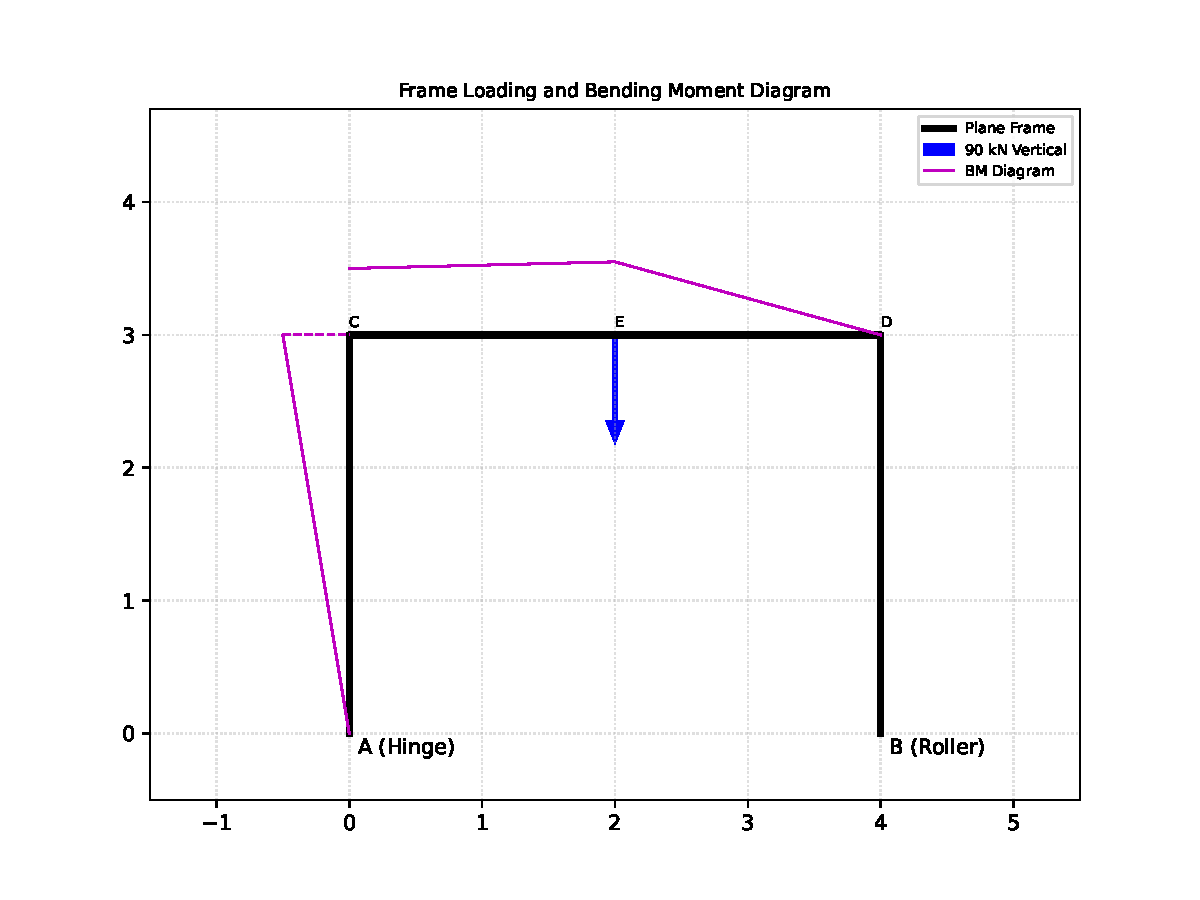
\includegraphics[width=0.7\linewidth]{figs/q39.pdf}
    \caption{Frame loading and bending moment diagram}
    \label{fig:q39}
\end{figure}

\begin{lstlisting}[frame=single, basicstyle=\rmfamily\small, breaklines=true, linewidth=\linewidth, escapeinside={(*@}{@*)}]
(*@\makebox[\dimexpr\linewidth-2\fboxsep-2\fboxrule\relax][c]{\parbox{\linewidth}{\centering codes/ce1q39/q39.py}}@*)
\end{lstlisting}

\begin{lstlisting}[frame=single, basicstyle=\rmfamily\small, breaklines=true, linewidth=\linewidth, escapeinside={(*@}{@*)}]
(*@\makebox[\dimexpr\linewidth-2\fboxsep-2\fboxrule\relax][c]{\parbox{\linewidth}{\centering codes/ce1q39/q39plot.py}}@*)
\end{lstlisting}
% ----------------------------------------------------------- Q48
\item Starting with the first approximation as $x = 0.5$, the second approximation for the root of the following function by the Newton-Raphson method is \underline{\hspace{2cm}} (rounded off to two decimal places).
\begin{align}
f\brak{x} = e^{-x} - x
\end{align}
\gate

\solution The function and its derivative are
\begin{align}
f\brak{x} &= e^{-x} - x\\
f'\brak{x} &= -e^{-x} - 1
\end{align}
Substituting into \eqref{eq:nr}:
\begin{align}
x_{n+1} &= x_n + \frac{e^{-x_n} - x_n}{e^{-x_n} + 1}\\
&= \frac{1 + x_n}{1 + e^{x_n}}
\end{align}
With the first approximation $x_0 = 0.5$, the second approximation is
\begin{align}
x_1 = \frac{1.5}{1 + e^{0.5}} = \frac{1.5}{2.64872} = 0.56631 \approx 0.57
\end{align}
Subsequent iterations converge to $x_2 = x_3 = 0.567143$.

\begin{figure}[H]
\centering
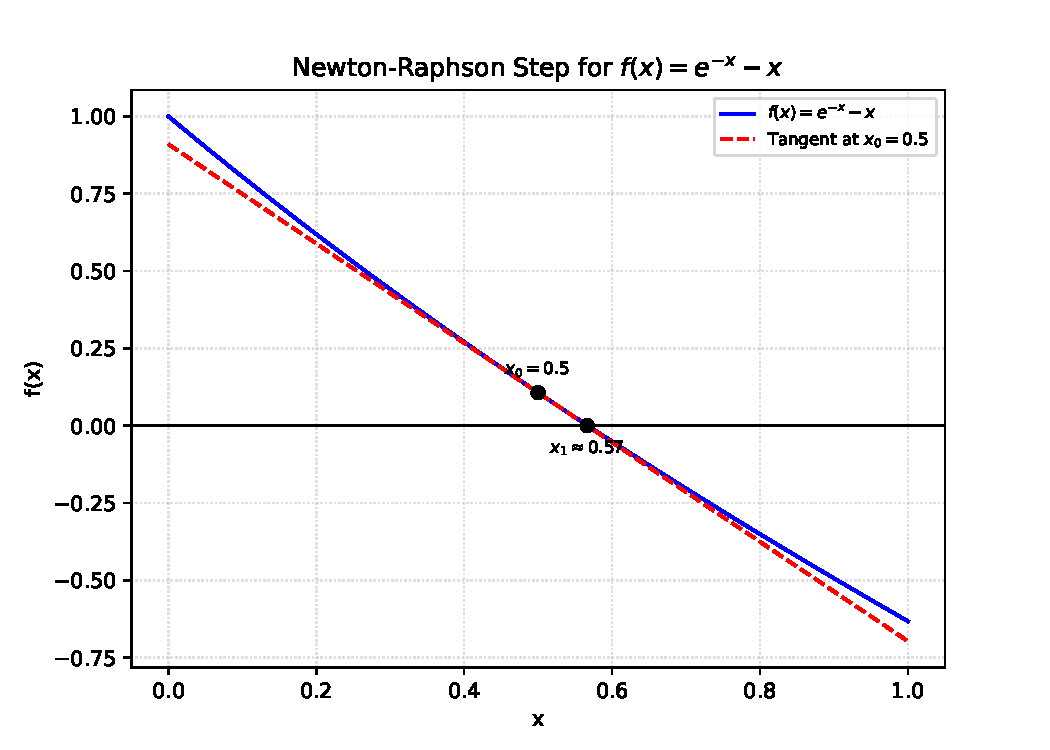
\includegraphics[width=0.7\columnwidth,keepaspectratio]{figs/q48.pdf}
\caption{One Newton-Raphson step for $f\brak{x} = e^{-x} - x$ from $x_0 = 0.5$}
\end{figure}
\begin{lstlisting}[frame=single, basicstyle=\rmfamily, escapeinside={(*@}{@*)}]
(*@\makebox[\dimexpr\linewidth-2\fboxsep-2\fboxrule\relax][c]{codes/ce1q48/q48.py}@*)
\end{lstlisting}
\begin{lstlisting}[frame=single, basicstyle=\rmfamily, escapeinside={(*@}{@*)}]
(*@\makebox[\dimexpr\linewidth-2\fboxsep-2\fboxrule\relax][c]{codes/ce1q48/q48plot.py}@*)
\end{lstlisting}

\begin{lstlisting}[frame=single, basicstyle=\rmfamily, escapeinside={(*@}{@*)}]
(*@\makebox[\dimexpr\linewidth-2\fboxsep-2\fboxrule\relax][c]{codes/ce1q48/q48.c}@*)
\end{lstlisting}


% ----------------------------------------------------------- Q49
\item Values of $y$ for different values of $x$ are tabulated below.
\begin{center}
\begin{tabular}{|c|c|c|c|}
\hline
$x$ & $-2$ & 1 & 2\\ \hline
$y$ & 28 & 4 & 16\\ \hline
\end{tabular}
\end{center}
If a second-degree interpolating polynomial $P_2\brak{x}$ is used to represent $y$, the value of $P_2\brak{0}$ is \underline{\hspace{2cm}} (rounded off to the nearest integer). \gate

\solution Let $\vec{c} = \myvec{c_0 & c_1 & c_2}^\top$ and $\vec{y} = \myvec{28 & 4 & 16}^\top$. From \eqref{eq:vander},
\begin{align}
\myvec{1 & -2 & 4\\ 1 & 1 & 1\\ 1 & 2 & 4}\vec{c} = \vec{y}
\end{align}
Reducing the augmented matrix:
\begin{align}
\myvec{1 & -2 & 4 & 28\\ 1 & 1 & 1 & 4\\ 1 & 2 & 4 & 16}
&\xrightarrow[R_3\to R_3 - R_1]{R_2\to R_2 - R_1}
\myvec{1 & -2 & 4 & 28\\ 0 & 3 & -3 & -24\\ 0 & 4 & 0 & -12}\\
&\implies c_1 = -3,\ c_2 = 5,\ c_0 = 2
\end{align}
Thus,
\begin{align}
\vec{c} = \myvec{2\\ -3\\ 5} \implies P_2\brak{x} = 5x^2 - 3x + 2
\end{align}
and
\begin{align}
P_2\brak{0} = \myvec{1 & 0 & 0}\vec{c} = 2
\end{align}

\begin{figure}[H]
\centering

\includegraphics[width=0.7\columnwidth,keepaspectratio]{figs/q49.pdf}
\caption{Interpolating polynomial through the given points}
\end{figure}
\begin{lstlisting}[frame=single, basicstyle=\rmfamily, escapeinside={(*@}{@*)}]
(*@\makebox[\dimexpr\linewidth-2\fboxsep-2\fboxrule\relax][c]{codes/ce1q49/q49.py}@*)
\end{lstlisting}
\begin{lstlisting}[frame=single, basicstyle=\rmfamily, escapeinside={(*@}{@*)}]
(*@\makebox[\dimexpr\linewidth-2\fboxsep-2\fboxrule\relax][c]{codes/ce1q49/q49plot.py}@*)
\end{lstlisting}

% ----------------------------------------------------------- Q50
\item Two identical blocks $A$ and $B$ are connected by a rigid rod. The blocks rest against vertical and horizontal planes, as shown in the figure. The coefficient of static friction at the vertical and horizontal planes is the same. If the sliding impends when $\theta = 45^\circ$, the value of the coefficient of static friction is \underline{\hspace{2cm}} (rounded off to two decimal places). \gate


\begin{center}
\begin{tikzpicture}[scale=1.2]

    % Define colors
    \definecolor{boxblue}{RGB}{20, 45, 85}

    % --- Hatching / Fixed Walls ---
    % Vertical Wall Hatching (Left)
    \fill[pattern=north east lines] (-0.25, 0) rectangle (0, 4.2);
    
    % Horizontal Floor Hatching (Bottom)
    \fill[pattern=north east lines] (-0.25, -0.25) rectangle (5.2, 0);

    % Solid Wall Surfaces
    \draw[line width=1.2pt, boxblue] (0, 4.2) -- (0, 0) -- (5.2, 0);

    % --- Block A (Top Left) ---
    % Outline & Fill
    \draw[line width=1.5pt, boxblue, fill=white] (0, 2.6) rectangle (1.0, 3.6);
    \coordinate (A) at (0.5, 3.1);
    
    % Label A and Pin Joint
    \node[anchor=south] at (0.5, 3.1) {\large\bfseries A};
    \fill[black] (A) circle (3.5pt);

    % --- Block B (Bottom Right) ---
    % Outline & Fill
    \draw[line width=1.5pt, boxblue, fill=white] (3.8, 0) rectangle (4.8, 1.0);
    \coordinate (B) at (4.3, 0.5);
    
    % Label B and Pin Joint
    \node[anchor=north] at (4.3, 0.5) {\large\bfseries B};
    \fill[black] (B) circle (3.5pt);

    % --- Connecting Rod ---
    \draw[line width=1.5pt, black] (A) -- (B);

    % --- Dashed Reference Line & Angle Theta ---
    % Midpoint of rod
    \coordinate (M) at ($(A)!0.52!(B)$);
    
    % Horizontal dashed line
    \draw[line width=1.2pt, dashed] ($(M)+(-1.2,0)$) -- ($(M)+(1.2,0)$);

    % Angle arc
    \draw[line width=1pt] (M) ++(180:0.6) arc (180:145.6:0.6);
    \node at ($(M) + (163:0.9)$) {\large $\mathbf{\theta}$};

\end{tikzpicture}
\end{center}
\solution Let each block have weight $W$ and let the rod make angle $\theta$ with the horizontal, with $c = \cos\theta$, $s = \sin\theta$. The rod is a two-force member carrying compression $C$ along
\begin{align}
\vec{e} = \frac{\vec{A} - \vec{B}}{\norm{\vec{A} - \vec{B}}} = \myvec{-c\\ s}
\end{align}
When sliding impends, $A$ moves down and $B$ moves away from the wall, so the friction forces are $\mu N_A$ (upward on $A$) and $\mu N_B$ (towards the wall on $B$). From \eqref{eq:equil}:
\begin{align}
\text{Block }A:&\quad \myvec{N_A\\ \mu N_A} + \myvec{0\\ -W} + C\myvec{-c\\ s} = \vec{0}\\
\text{Block }B:&\quad \myvec{-\mu N_B\\ N_B} + \myvec{0\\ -W} - C\myvec{-c\\ s} = \vec{0}
\end{align}
This gives four equations in three unknowns $\myvec{N_A & N_B & C}^\top$:
\begin{align}
\myvec{1 & 0 & -c\\ \mu & 0 & s\\ 0 & -\mu & c\\ 0 & 1 & -s}\myvec{N_A\\ N_B\\ C} = \myvec{0\\ W\\ 0\\ W}
\end{align}
From \eqref{eq:augdet}, the system is consistent only if
\begin{align}
\mydet{1 & 0 & -c & 0\\ \mu & 0 & s & W\\ 0 & -\mu & c & 0\\ 0 & 1 & -s & W} = 0
\end{align}
Expanding along the second column,
\begin{align}
\mu\mydet{1 & -c & 0\\ \mu & s & W\\ 0 & -s & W} + \mydet{1 & -c & 0\\ \mu & s & W\\ 0 & c & 0} &= 0\\
\mu W\brak{2s + \mu c} - Wc &= 0\\
\implies \tan\theta &= \frac{1 - \mu^2}{2\mu}
\end{align}
For $\theta = 45^\circ$:
\begin{align}
\mu^2 + 2\mu - 1 = 0 \implies \mu = -1 + \sqrt{2} = 0.414
\end{align}
taking the positive root.

\begin{figure}[H]
\centering
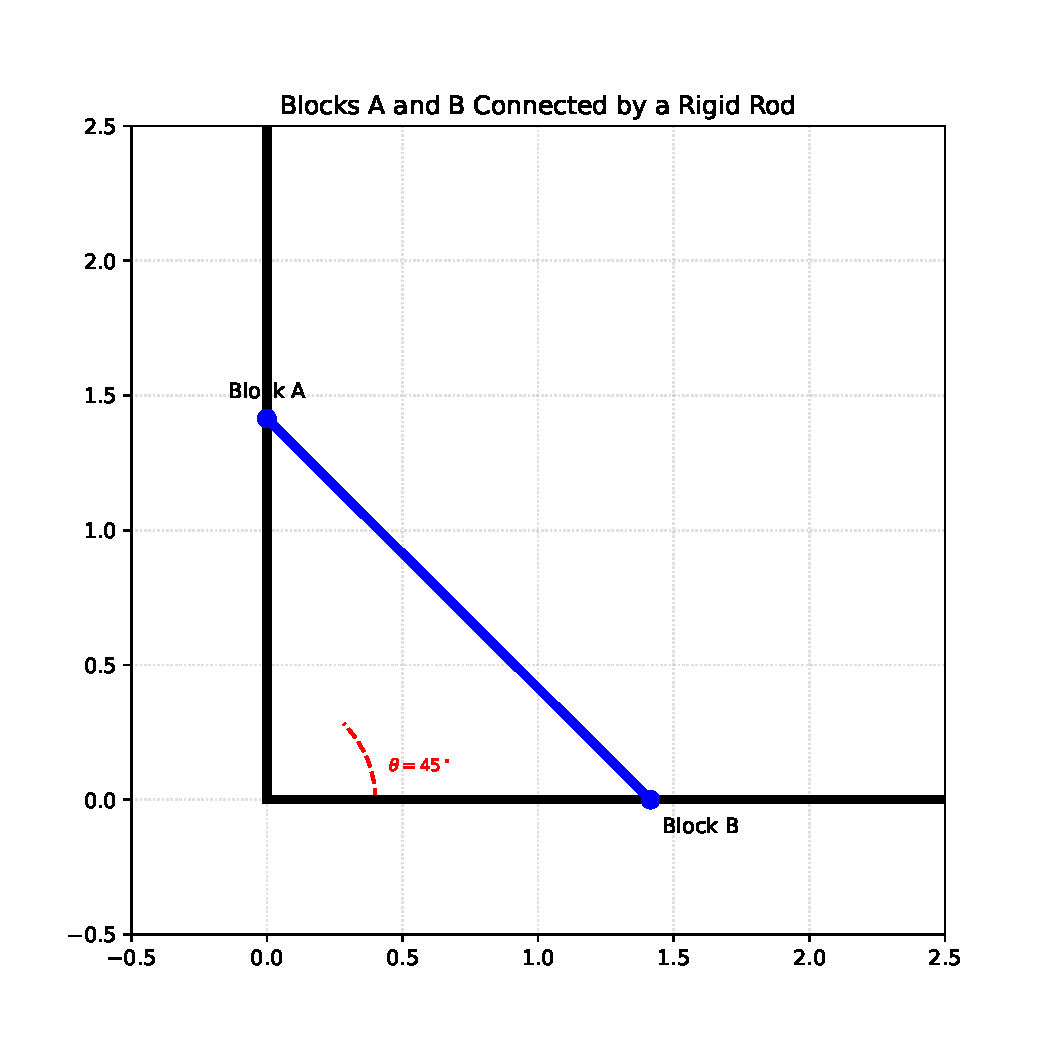
\includegraphics[width=0.7\columnwidth,keepaspectratio]{figs/q50.pdf}
\caption{Blocks $A$ and $B$ connected by a rigid rod at $\theta = 45^\circ$}
\end{figure}
\begin{lstlisting}[frame=single, basicstyle=\rmfamily, escapeinside={(*@}{@*)}]
(*@\makebox[\dimexpr\linewidth-2\fboxsep-2\fboxrule\relax][c]{codes/ce1q50/q50.py}@*)
\end{lstlisting}
\begin{lstlisting}[frame=single, basicstyle=\rmfamily, escapeinside={(*@}{@*)}]
(*@\makebox[\dimexpr\linewidth-2\fboxsep-2\fboxrule\relax][c]{codes/ce1q50/q50plot.py}@*)
\end{lstlisting}

% ----------------------------------------------------------- Q51
\item A homogenous, linearly elastic rod $AB$ is connected to a linearly elastic spring $BC$ in between the fixed supports at $A$ and $C$, as shown in the figure. The cross-sectional area, modulus of elasticity, and the coefficient of thermal expansion of the rod $AB$ are 500 mm$^2$, $60\times 10^3$ MPa, and $12\times 10^{-6}$ per $^\circ$C, respectively. The stiffness $\brak{k}$ of spring $BC$ is 2500 N/mm.

The internal force (in kN) that will develop in the spring $BC$ when the temperature of rod $AB$ is increased by $100^\circ$C is \underline{\hspace{2cm}} (rounded off to one decimal place). \gate

\begin{center}
\begin{tikzpicture}[scale=1.2]

    % --- Left Wall (A) ---
    \fill[pattern=north east lines] (-0.35, -0.2) rectangle (0, 1.0);
    \draw[line width=1.2pt] (0, -0.2) -- (0, 1.0);

    % --- Bar AB ---
    \draw[line width=1.5pt] (0, 0) rectangle (4, 0.8);

    % --- Spring BC ---
    \draw[line width=1.2pt] (4, 0.4) -- (4.2, 0.4);
    \draw[line width=1.2pt, decorate, decoration={coil, aspect=0.5, segment length=3.5mm, amplitude=2.8mm}] (4.2, 0.4) -- (6.8, 0.4);
    \draw[line width=1.2pt] (6.8, 0.4) -- (7.0, 0.4);

    % --- Right Wall (C) ---
    \fill[pattern=north east lines] (7.0, -0.2) rectangle (7.35, 1.0);
    \draw[line width=1.2pt] (7.0, -0.2) -- (7.0, 1.0);

    % --- Node Labels ---
    \node[anchor=north west, font=\bfseries\large] at (0, -0.02) {A};
    \node[anchor=north east, font=\bfseries\large] at (4, -0.02) {B};
    \node[anchor=north east, font=\bfseries\large] at (7, -0.02) {C};

    % --- Spring Stiffness Label ---
    \node[above, font=\bfseries\large] at (5.5, 0.8) {k = 2500 N/mm};

    % --- Dimension Line (3 m) ---
    % Vertical extension ticks
    \draw[line width=1.2pt] (0, 1.3) -- (0, 2.1);
    \draw[line width=1.2pt] (4, 1.3) -- (4, 2.1);
    
    % Diagonal slash ticks
    \draw[line width=1.2pt] (-0.2, 1.5) -- (0.2, 1.9);
    \draw[line width=1.2pt] (3.8, 1.5) -- (4.2, 1.9);
    
    % Horizontal dimension line with arrows
    \draw[line width=1.2pt, <->, >=Stealth] (0, 1.7) -- (4, 1.7) 
        node[midway, above, font=\bfseries\large] {3 m};

    % --- Note at Bottom ---
    \node[font=\bfseries\large] at (3.5, -1.2) {(Figure not to scale)};

\end{tikzpicture}
\end{center}

\solution From the figure, the length of rod $AB$ is $L = 3$ m $= 3000$ mm. The rod stiffness  \eqref{eq:kbar} is
\begin{align}
k_r = \frac{AE}{L} = \frac{500\times 60\times 10^3}{3000} = 10^4\text{ N/mm} = 10000\text{ N/mm}
\end{align}
The free thermal expansion  \eqref{eq:free} of the rod is
\begin{align}
\delta_{\text{th}} = L\alpha\Delta T = 3000 \times 12\times 10^{-6} \times 100 = 3.6\text{ mm}
\end{align}
Since the rod and spring are in series between fixed supports, the internal compressive force $F$ satisfies
\begin{align}
\frac{F}{k_r} + \frac{F}{k_s} = \delta_{\text{th}} \implies F = \frac{\delta_{\text{th}}}{\frac{1}{k_r} + \frac{1}{k_s}}
\end{align}
Substituting $k_r = 10000\text{ N/mm}$ and $k_s = 2500\text{ N/mm}$:
\begin{align}
F = \frac{3.6}{\frac{1}{10000} + \frac{1}{2500}} = \frac{3.6}{0.0005} = 7200\text{ N} = 7.2\text{ kN}
\end{align}

\begin{figure}[H]
\centering

\includegraphics[width=0.7\columnwidth,keepaspectratio]{figs/q51.pdf}
\caption{Rod $AB$ connected in series with spring $BC$ under thermal loading}
\end{figure}
\begin{lstlisting}[frame=single, basicstyle=\rmfamily, escapeinside={(*@}{@*)}]
(*@\makebox[\dimexpr\linewidth-2\fboxsep-2\fboxrule\relax][c]{codes/ce1q51/q51.py}@*)
\end{lstlisting}
\begin{lstlisting}[frame=single, basicstyle=\rmfamily, escapeinside={(*@}{@*)}]
(*@\makebox[\dimexpr\linewidth-2\fboxsep-2\fboxrule\relax][c]{codes/ce1q51/q51plot.py}@*)
\end{lstlisting}

\end{enumerate}
